\documentclass[crop,tikz]{standalone}

\usetikzlibrary{
	chains,
	positioning,
	arrows.meta,
	decorations.pathreplacing,
	calc,
	fit,
	shapes.geometric
}

\begin{document}

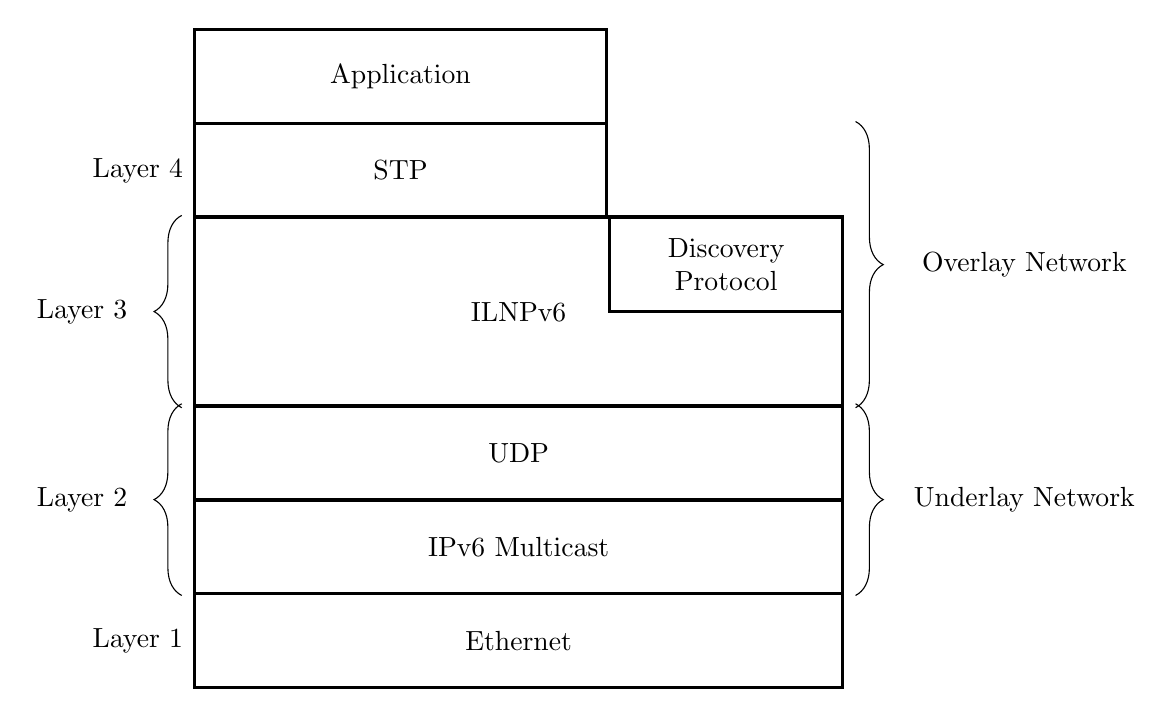
\begin{tikzpicture}[
	node distance = -0.5mm and 0mm,
	start chain = going below,
	layer/.style args = {#1}{
		rectangle, draw, very thick,
		text width=8cm, align=center,
		minimum height=12mm,
		label=left:#1
	}
]

	\node (n3) [layer={}, on chain, minimum height=24mm] {ILNPv6};
		\node (n4) [layer={Layer 4},above right=of n3.north west,text width=5cm] {STP};
		\node (n5) [layer={},above right=of n4.north west,text width=5cm] {Application};
		\node (n3B) [layer=,below left=0pt and 0pt of n3.north east,text width=2.73cm] {Discovery Protocol};
		\node (n4B) [layer=,above left=of n3B.north east,text width=2cm,draw=none] {};
		\node (n5B) [layer=,above left=of n4B.north east,text width=2cm,draw=none] {};
	
	\node (n2) [layer, on chain] {UDP};
	\node (n1) [layer, on chain] {IPv6 Multicast};
	\node (n0) [layer={Layer 1}, on chain] {Ethernet};
	
	\draw [decorate, decoration={brace, amplitude=10pt, raise=4pt, mirror}]
		(n3.south east) -- (n4B.north east)
		node [black, midway, xshift=65pt] {Overlay Network};
	
	\draw [decorate, decoration={brace, amplitude=10pt, raise=4pt, mirror}]
		(n1.south east) -- (n2.north east)
		node [black, midway, xshift=65pt] {Underlay Network};
	
	\draw [decorate, decoration={brace, amplitude=10pt, raise=4pt}]
		(n1.south west) -- (n2.north west)
		node [black, midway, xshift=-40pt] {Layer 2};
	
	\draw [decorate, decoration={brace, amplitude=10pt, raise=4pt}]
		(n3.south west) -- (n3.north west)
		node [black, midway, xshift=-40pt] {Layer 3};
\end{tikzpicture}

\end{document}